% Created by tikzDevice version 0.12.6 on 2025-01-14 08:13:27
% !TEX encoding = UTF-8 Unicode
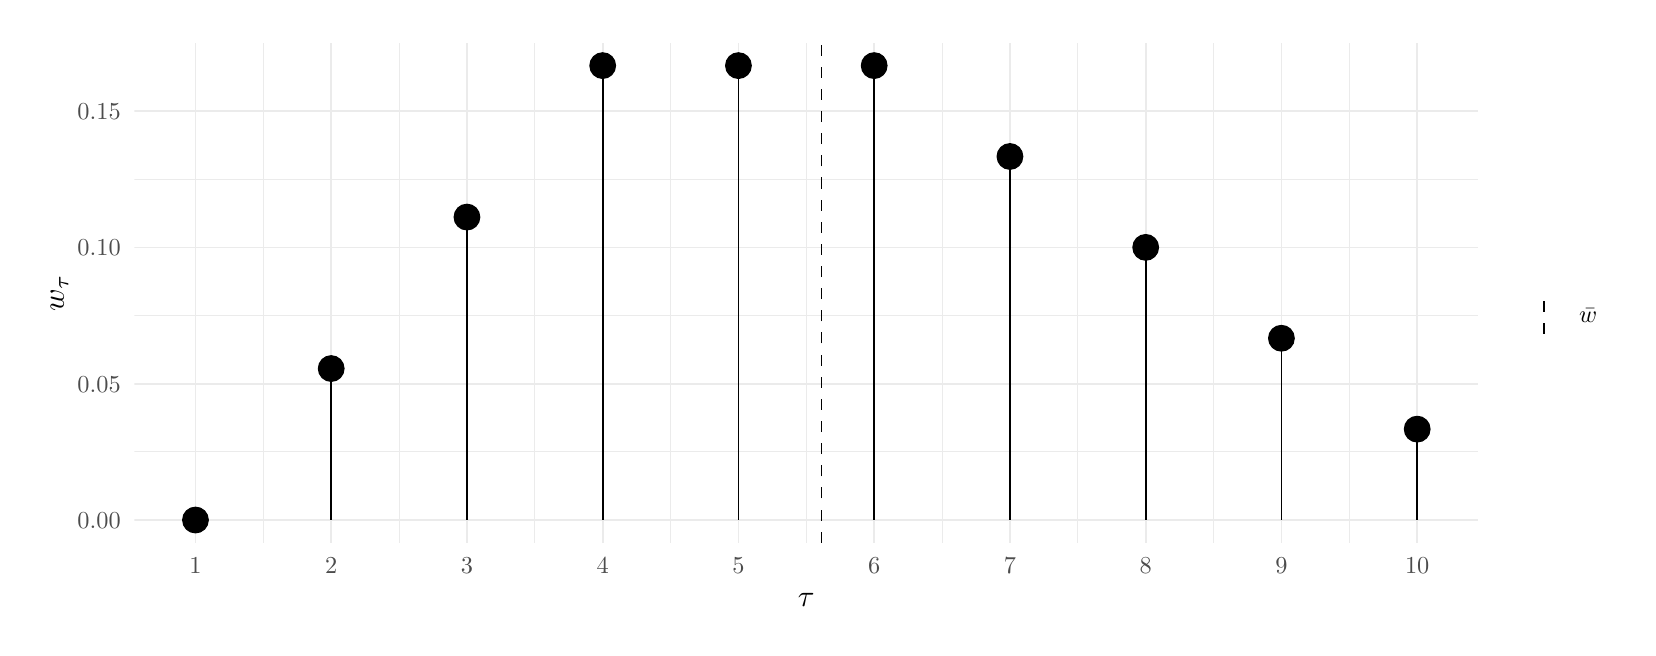
\begin{tikzpicture}[x=1pt,y=1pt]
\definecolor{fillColor}{RGB}{255,255,255}
\path[use as bounding box,fill=fillColor,fill opacity=0.00] (0,0) rectangle (578.16,216.81);
\begin{scope}
\path[clip] ( 38.56, 30.69) rectangle (524.17,211.31);
\definecolor{drawColor}{gray}{0.92}

\path[draw=drawColor,line width= 0.3pt,line join=round] ( 38.56, 63.53) --
	(524.17, 63.53);

\path[draw=drawColor,line width= 0.3pt,line join=round] ( 38.56,112.79) --
	(524.17,112.79);

\path[draw=drawColor,line width= 0.3pt,line join=round] ( 38.56,162.05) --
	(524.17,162.05);

\path[draw=drawColor,line width= 0.3pt,line join=round] ( 85.15, 30.69) --
	( 85.15,211.31);

\path[draw=drawColor,line width= 0.3pt,line join=round] (134.21, 30.69) --
	(134.21,211.31);

\path[draw=drawColor,line width= 0.3pt,line join=round] (183.26, 30.69) --
	(183.26,211.31);

\path[draw=drawColor,line width= 0.3pt,line join=round] (232.31, 30.69) --
	(232.31,211.31);

\path[draw=drawColor,line width= 0.3pt,line join=round] (281.36, 30.69) --
	(281.36,211.31);

\path[draw=drawColor,line width= 0.3pt,line join=round] (330.41, 30.69) --
	(330.41,211.31);

\path[draw=drawColor,line width= 0.3pt,line join=round] (379.47, 30.69) --
	(379.47,211.31);

\path[draw=drawColor,line width= 0.3pt,line join=round] (428.52, 30.69) --
	(428.52,211.31);

\path[draw=drawColor,line width= 0.3pt,line join=round] (477.57, 30.69) --
	(477.57,211.31);

\path[draw=drawColor,line width= 0.6pt,line join=round] ( 38.56, 38.90) --
	(524.17, 38.90);

\path[draw=drawColor,line width= 0.6pt,line join=round] ( 38.56, 88.16) --
	(524.17, 88.16);

\path[draw=drawColor,line width= 0.6pt,line join=round] ( 38.56,137.42) --
	(524.17,137.42);

\path[draw=drawColor,line width= 0.6pt,line join=round] ( 38.56,186.68) --
	(524.17,186.68);

\path[draw=drawColor,line width= 0.6pt,line join=round] ( 60.63, 30.69) --
	( 60.63,211.31);

\path[draw=drawColor,line width= 0.6pt,line join=round] (109.68, 30.69) --
	(109.68,211.31);

\path[draw=drawColor,line width= 0.6pt,line join=round] (158.73, 30.69) --
	(158.73,211.31);

\path[draw=drawColor,line width= 0.6pt,line join=round] (207.78, 30.69) --
	(207.78,211.31);

\path[draw=drawColor,line width= 0.6pt,line join=round] (256.84, 30.69) --
	(256.84,211.31);

\path[draw=drawColor,line width= 0.6pt,line join=round] (305.89, 30.69) --
	(305.89,211.31);

\path[draw=drawColor,line width= 0.6pt,line join=round] (354.94, 30.69) --
	(354.94,211.31);

\path[draw=drawColor,line width= 0.6pt,line join=round] (403.99, 30.69) --
	(403.99,211.31);

\path[draw=drawColor,line width= 0.6pt,line join=round] (453.04, 30.69) --
	(453.04,211.31);

\path[draw=drawColor,line width= 0.6pt,line join=round] (502.10, 30.69) --
	(502.10,211.31);
\definecolor{drawColor}{RGB}{0,0,0}
\definecolor{fillColor}{RGB}{0,0,0}

\path[draw=drawColor,line width= 0.4pt,line join=round,line cap=round,fill=fillColor] ( 60.63, 38.90) circle (  4.64);

\path[draw=drawColor,line width= 0.4pt,line join=round,line cap=round,fill=fillColor] (109.68, 93.63) circle (  4.64);

\path[draw=drawColor,line width= 0.4pt,line join=round,line cap=round,fill=fillColor] (158.73,148.37) circle (  4.64);

\path[draw=drawColor,line width= 0.4pt,line join=round,line cap=round,fill=fillColor] (207.78,203.10) circle (  4.64);

\path[draw=drawColor,line width= 0.4pt,line join=round,line cap=round,fill=fillColor] (256.84,203.10) circle (  4.64);

\path[draw=drawColor,line width= 0.4pt,line join=round,line cap=round,fill=fillColor] (305.89,203.10) circle (  4.64);

\path[draw=drawColor,line width= 0.4pt,line join=round,line cap=round,fill=fillColor] (354.94,170.26) circle (  4.64);

\path[draw=drawColor,line width= 0.4pt,line join=round,line cap=round,fill=fillColor] (403.99,137.42) circle (  4.64);

\path[draw=drawColor,line width= 0.4pt,line join=round,line cap=round,fill=fillColor] (453.04,104.58) circle (  4.64);

\path[draw=drawColor,line width= 0.4pt,line join=round,line cap=round,fill=fillColor] (502.10, 71.74) circle (  4.64);

\path[draw=drawColor,line width= 0.6pt,line join=round] ( 60.63, 38.90) -- ( 60.63, 38.90);

\path[draw=drawColor,line width= 0.6pt,line join=round] (109.68, 93.63) -- (109.68, 38.90);

\path[draw=drawColor,line width= 0.6pt,line join=round] (158.73,148.37) -- (158.73, 38.90);

\path[draw=drawColor,line width= 0.6pt,line join=round] (207.78,203.10) -- (207.78, 38.90);

\path[draw=drawColor,line width= 0.6pt,line join=round] (256.84,203.10) -- (256.84, 38.90);

\path[draw=drawColor,line width= 0.6pt,line join=round] (305.89,203.10) -- (305.89, 38.90);

\path[draw=drawColor,line width= 0.6pt,line join=round] (354.94,170.26) -- (354.94, 38.90);

\path[draw=drawColor,line width= 0.6pt,line join=round] (403.99,137.42) -- (403.99, 38.90);

\path[draw=drawColor,line width= 0.6pt,line join=round] (453.04,104.58) -- (453.04, 38.90);

\path[draw=drawColor,line width= 0.6pt,line join=round] (502.10, 71.74) -- (502.10, 38.90);

\path[draw=drawColor,line width= 0.6pt,dash pattern=on 4pt off 4pt ,line join=round] (286.81, 30.69) -- (286.81,211.31);
\end{scope}
\begin{scope}
\path[clip] (  0.00,  0.00) rectangle (578.16,216.81);
\definecolor{drawColor}{gray}{0.30}

\node[text=drawColor,anchor=base east,inner sep=0pt, outer sep=0pt, scale=  0.88] at ( 33.61, 35.87) {0.00};

\node[text=drawColor,anchor=base east,inner sep=0pt, outer sep=0pt, scale=  0.88] at ( 33.61, 85.13) {0.05};

\node[text=drawColor,anchor=base east,inner sep=0pt, outer sep=0pt, scale=  0.88] at ( 33.61,134.39) {0.10};

\node[text=drawColor,anchor=base east,inner sep=0pt, outer sep=0pt, scale=  0.88] at ( 33.61,183.65) {0.15};
\end{scope}
\begin{scope}
\path[clip] (  0.00,  0.00) rectangle (578.16,216.81);
\definecolor{drawColor}{gray}{0.30}

\node[text=drawColor,anchor=base,inner sep=0pt, outer sep=0pt, scale=  0.88] at ( 60.63, 19.68) {1};

\node[text=drawColor,anchor=base,inner sep=0pt, outer sep=0pt, scale=  0.88] at (109.68, 19.68) {2};

\node[text=drawColor,anchor=base,inner sep=0pt, outer sep=0pt, scale=  0.88] at (158.73, 19.68) {3};

\node[text=drawColor,anchor=base,inner sep=0pt, outer sep=0pt, scale=  0.88] at (207.78, 19.68) {4};

\node[text=drawColor,anchor=base,inner sep=0pt, outer sep=0pt, scale=  0.88] at (256.84, 19.68) {5};

\node[text=drawColor,anchor=base,inner sep=0pt, outer sep=0pt, scale=  0.88] at (305.89, 19.68) {6};

\node[text=drawColor,anchor=base,inner sep=0pt, outer sep=0pt, scale=  0.88] at (354.94, 19.68) {7};

\node[text=drawColor,anchor=base,inner sep=0pt, outer sep=0pt, scale=  0.88] at (403.99, 19.68) {8};

\node[text=drawColor,anchor=base,inner sep=0pt, outer sep=0pt, scale=  0.88] at (453.04, 19.68) {9};

\node[text=drawColor,anchor=base,inner sep=0pt, outer sep=0pt, scale=  0.88] at (502.10, 19.68) {10};
\end{scope}
\begin{scope}
\path[clip] (  0.00,  0.00) rectangle (578.16,216.81);
\definecolor{drawColor}{RGB}{0,0,0}

\node[text=drawColor,anchor=base,inner sep=0pt, outer sep=0pt, scale=  1.10] at (281.36,  7.64) {$\tau$};
\end{scope}
\begin{scope}
\path[clip] (  0.00,  0.00) rectangle (578.16,216.81);
\definecolor{drawColor}{RGB}{0,0,0}

\node[text=drawColor,rotate= 90.00,anchor=base,inner sep=0pt, outer sep=0pt, scale=  1.10] at ( 13.08,121.00) {$w_\tau$};
\end{scope}
\begin{scope}
\path[clip] (  0.00,  0.00) rectangle (578.16,216.81);
\definecolor{drawColor}{RGB}{0,0,0}

\path[draw=drawColor,line width= 0.6pt,dash pattern=on 4pt off 4pt ,line join=round] (547.90,106.16) -- (547.90,120.62);
\end{scope}
\begin{scope}
\path[clip] (  0.00,  0.00) rectangle (578.16,216.81);
\definecolor{drawColor}{RGB}{0,0,0}

\node[text=drawColor,anchor=base west,inner sep=0pt, outer sep=0pt, scale=  0.88] at (560.62,110.36) {$\bar w$};
\end{scope}
\end{tikzpicture}
